\documentclass[11pt, a4paper]{article}
\usepackage{graphicx, fullpage, hyperref, listings}
\usepackage{appendix, pdfpages, color}
\usepackage{indentfirst} %段首空两格 棒
\usepackage{chngpage} 
\usepackage{tocloft}            % This squashes the Table of Contents a bit
\usepackage{pdfpages}
\usepackage{multirow}
\usepackage{amsmath}
\usepackage{framed}


\setlength\cftbeforesecskip{3pt}
\renewcommand{\contentsname}{\centerline{\textbf{Content}}}
\graphicspath{{images/}}

\usepackage{multicol}

\usepackage{graphicx}
\usepackage{epstopdf}
\hypersetup{CJKbookmarks,%
	bookmarksnumbered,%
	colorlinks,%
	linkcolor=black,%
	citecolor=black,%
	plainpages=false,%
	pdfstartview=FitH}

%%%%%%%代码语法高亮设置

\usepackage{color}

\definecolor{pblue}{rgb}{0.13,0.13,1}
\definecolor{pgreen}{rgb}{0,0.5,0}
\definecolor{pred}{rgb}{0.9,0,0}
\definecolor{pgrey}{rgb}{0.46,0.45,0.48}

\usepackage{listings}
\lstset{
	language=Java,
	showspaces=false,
	showtabs=false,
	%%%%%
	frame = single,
	stepnumber = 2,  
	numbersep = 4pt, 
	 numbers=left,
	%breakatwhitespace=false, 
	tabsize=2,  
	%%%%%
	breaklines=true,
	showstringspaces=false,
    breakatwhitespace=false, 
	commentstyle=\color{pgreen},
	keywordstyle=\color{pblue},
	stringstyle=\color{pred},
	basicstyle=\ttfamily,
	%moredelim=[il][\textcolor{pgrey}]{$$},
	%moredelim=[is][\textcolor{pgrey}]{\%\%}{\%\%},
}


%%%%%%%%代码语法高亮设置

\definecolor{MyLightYellow}{cmyk}{0,0.,0.2,0} 

\setlength{\parskip}{4pt}        % sets spacing between paragraphs
\interfootnotelinepenalty=500    % this prevents footnotes breaking across pages

\title{
\includegraphics[width=0.45\textwidth]{wpi2}
        \\CS 534 Artificial Intelligence Final Project \\ GoBang Game Project Report}          % <<<<<<<<< change the title as appropriate
\author{Group 10 }                    % <<<<<<<<< module code

\begin{document}
\begin{titlepage}
	
%\date{\today}
\maketitle
\addtocontents{toc}{\protect\thispagestyle{empty}} % because we don't want a page number on the title page
% Thanks to Huang Shanyue for suggesting this 

\begin{center}
Group Member
\end{center}

\begin{table}[htbp] 
\begin{center}
\begin{tabular}{l l l} 
	 
	 
	 Yixuan & Jiao  &   yjiao@wpi.edu \\
     Yinkai & Ma  &   yma7@wpi.edu \\
     Fangling & Zhang  & fzhang2@wpi.edu         \\
     Jiaming & Nie  &  jnie@wpi.edu \\
     Pinyi & Xiao  &  pxiao@wpi.edu \\
\end{tabular}
\end{center}
\end{table}



%\date{\today}
\thispagestyle{empty}  %去除首页页码

\end{titlepage}

\tableofcontents
%\listoffigures

\newpage

\section{Introduction}

\subsection{Basic Rule}

Gobang Game, is also called Gomoku, FIR (Five in a Row). The traditional Gobang game uses the same game board and pieces as Go. There are two players, black and white. Players alternate turns placing a stone of his color on an empty intersection of the straight and horizontal lines. The first player who makes an unbroken chain of five stones horizontally, vertically, or diagonally, is the winner.
We can use tic-tac-toe to help us better understand the rule of Gobang Game. In general, Gobang Game is very similar to tic-tac-toe. They both require players to form an unbroken chain to win. The only differences are that Gobang Game:

\begin{itemize}
\item[1.] Uses larger board and more pieces than tic-tac-toe.
\item[2.] Uses black and white stones instead of O and X.
\item[3.] Places pieces on the intersections but not in the grid.
\item[4.] (The most important) Requires "five-pieces" chain to win.

\end{itemize}

Being compared with tic-tac-toe, Gobang is played on a larger game board, thus there will be more special situations need to be considered during the play of Gobang Game. Learning these patterns can help us better understand the strategies for how to win the game. We will introduce these patterns in the following paragraph.

\subsection{Some Basic Patterns}

The board is very large, so there may be many possible patterns occur during the game. It is hard to conclude all the situations that may happen. Thus, here we only introduce some basic patterns (frequently used) to help us understand key threats and winning strategies during the game. In the following examples, '0' represents an empty space, '1' represents a black stone, and '2' represents a white stone.

\begin{itemize}
\item[1.] Consecutive Five. Five same color pieces in a row.
\item[2.] Open Four. A four-pieces chain that can form into a five-pieces chain by placing a piece on either side. Eg. 011110
\item[3.] Capped or Gapped Four. Only one place is available to form the four pieces into a five-pieces chain. Eg. 011112, 0101110, 0110110
\item[4.] Open Three. Three pieces that can be connected into 'Open Four'. Eg. 01110, 010110
\item[5.] Capped or Gapped Three. Three pieces that can be connected into 'Capped or Gapped Four'. Eg. 001112, 010112, 011012, 10011, 10101, 2011102
\item[6.] Open Two. Two pieces that can be connected into “Open Three”. Eg. 00110, 01010, 010010
\item[7.] Capped or Gapped Two. Two pieces that can be connected into “Capped or Gapped Four”. Eg. 000112, 001012, 010012, 10001, 2010102, 2011002
\item[8.] Double Four. The pattern that two four-pieces chains(either Open, or Capped or Gapped) can be formed by only placing one piece.
\item[9.] Four-Three. The pattern that a four-pieces chain(either Open, or Capped or Gapped) and a 'Open Three' can be formed at same time by only placing one piece.
\item[10.] Double Open Three. The pattern that two 'Open Three' chains can be formed by only placing one piece. Eg. Black pieces in figure 1.

\end{itemize}

\subsection{Computers and Gobang}

As Gobang is a chess game that be known mainly in asian area. So the progress on Gobang AI study is very slow. Currently, there isn’t a commercial Gobang AI program. The most strongest non-commercial Gobang AI is called Yixin, which is realized by Kai Sun, a CS Ph.D. in Cornell University. In average, Yixin takes 30 seconds to make decision on the next movement since 2016. Before 2016, It needs about 45 seconds in average to make decisions. In the most recent competition between Yixin and Qiguan, a human player of Gobang level six, Yixin had 1 win, 3 draw and 1 loss in 5 games. According to this result, we can infer that the intelligence level of current Gobang AI is similar to a sixth-level human player. However, the highest level of Gobang is level nine. Thus, there are still a lot to be improved in Gobang AI.


\section{Methodology}

\subsubsection{Goals and Purposes}

Currently, most of the Gobang AI are realized by using MiniMax with alpha-beta pruning. There are also some Gobang AI are realized by using Monte Carlo Tree Search(MCTS). As we all know, Gobang is in some extent similar to Go. However, majority people prefer to use MiniMax to realize Gobang, whereas use MCTS to realize Go. Thus, we want to know whether it’s more efficient to realize Gobang by using MiniMax. To find out the answer, we need to compare the performance of MiniMax and MCTS in Gobang AI. In general, we have two purposes for this project:

\begin{itemize}
\item[1.] We want to realize the Gobang AI. 
\item[2.] We want to compare the performances of MiniMax and Monte Carlo Tree Search in Gobang AI. 

\end{itemize}

\subsection{Milestones}

\begin{itemize}
\item[1.] Realize Gobang AI by using MiniMax with DFS and alpha-beta pruning.

\item[2.] Realize Gobang AI by using Monte Carlo Tree Search
\item[3.] Do experiments and compare the two methods.
\end{itemize}

Future vision: We can improve the Gobang AI performance by using the analysis in this project.

\subsection{Project Approaches}

At first, we will realize the Gobang AI by using two methods, MiniMax and Monte Carlo Tree Search(MCTS), respectively. We will also try to improve the efficiency of these approaches, for instance, applying alpha-beta pruning. After realizing the Gobang game with both approaches, we will do some experiments to compare these two approaches and find out the performance differences between each other. For example, we may ask the two AI fight against each other and find out that which method is more efficient, which one has a larger winning rate, and which one takes less time to make decisions. The detailed information on how we applied these two algorithms in Gobang will be explained in the following paragraphs.

\subsection{MiniMax}

Our AI algorithm is mainly designed on Minimax algorithm. Minimax is good at solving Zero-sum problems like Go-Bang. Two players are named as “Max” and “MIn”, “Max” always moves to the highest utility value node, while “Min” tends to move to the lowest utility value node. From the perspective of “Max”, the algorithm does Depth First Searching (DFS) from up to down, moving forward to the leaf nodes on the setted depth(3 layers in our algorithm) or bottom of the tree and find the heuristic utility values of them. Then it comes to the basic theory of this algorithm: supposing the rival “Min” will always make the choices which will gain the lowest utility value, and player “Max” will always take actions leading to the highest utility value basing on those choices. The algorithm will do this repeatedly until it send back an utility value to the root node finally.

The graph of the algorithm is illustrated in the figure on the following figure~\ref{Fig:mini-max}:

\begin{figure}[htbp]
	
	\centering %使插入的图片居中显示
	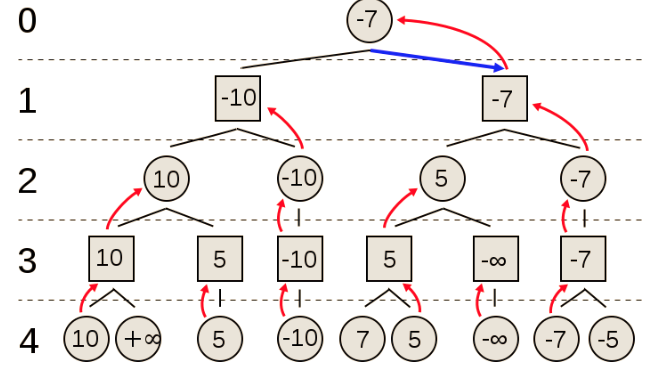
\includegraphics[width=10cm]{mini_max}
	
	\caption{Mini-Max Search}
	\label{Fig:mini-max}
	%插入图片的标题,一般放在图片的下方,放在表格的上方
	
\end{figure}

In the example, “Max” is supposed to take the biggest returned value while “Min” take the smallest returned value.

\subsubsection{Alpha-Beta Pruning}

The number of nodes that Minimax need to search is $O(b^m)$ which is a rather huge exponential value. So a pruning skill is essential to our design. We chose Alpha-Beta pruning for convenience. By applying this method to the Minimax tree, we can cut off those branches having no impact on the final decision.
In the Alpha-Beta pruning algorithm: “alpha” refers to the best choice of player “Max” on the route up till now; “beta” refers to the best choice of player “Min” on the route up till now.
The values of “alpha” and "beta" are upgraded during the searching process. And also, when the value of a node is worse than "alpha" or "beta", prun the rest branches of the node. The general theory of alpha-beta pruning is: When the player moves into node "n", if a better choice "m" exists in father node or upper nodes of node "n", then "n" will never be reached in a real game. So when we find the situation above, a pruning should be taken into action.

The Alpha-Beta search algorithm is on the following figure~\ref{Fig:ab}:

\begin{figure}[htbp]
	
	\centering %使插入的图片居中显示
	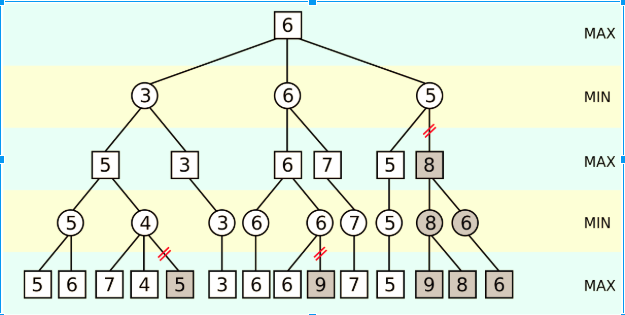
\includegraphics[width=10cm]{alpha_beta}
	
	\caption{Alpha-Beta Pruning}
	\label{Fig:ab}
	%插入图片的标题,一般放在图片的下方,放在表格的上方
	
\end{figure}

\subsection{Monte Carlo Tree Search}

We can use Monte Carlo Tree Search in any problem that can be described by {state, action}. The basic monte carlo tree search is very simple. However, the difficulty is that it’s hard to balance the exploration of simulation moves and the exploitation of deep successories when it reaches a high average win rate. The basic steps of MCTS is explained as following:


\begin{itemize}
\item Selection: start from root R and select successive child nodes down to a leaf node L. The essence of Monte Carlo tree search is the way to choose child nodes and promise the future expands make the “best” move.
\item Expansion: If L isn’t an ending node, then create one or more child nodes and select one node C among them.
\item Simulation: Run a simulated result from node C until the game ends. play a random playout from node C. This step is sometimes also called playout or rollout.
\item Backpropagation: Update current states(action sequence) by using the simulated results.

\end{itemize}

Each of the node must include the information of the estimated value of simulation result and the times it has been visited.

\subsubsection{Markov decision process}

Markov Decision Process is composed of four elements: (S, A, Psa, R, 𝛄), where “S” is the state, “A” is the action, “Psa” is the probability of taking action A in state S, “R” is the reward, “𝛄” is the discount factor that is defined between 0 and 1.

\subsubsection{Differences between UCB and e-greedy}

UCB is a more heuristic function while $\epsilon$ greedy algorithm performs higher speed.

\section{Results}

The results part will give the result for 2 kinds of the AI in the Go Bang game, which are based on the $\alpha-\beta$ pruning and the Monte Carlo tree search algorithms respectively.  

The program will take the inputs to choose the game mode.

\subsection{$\alpha-\beta$ Pruning Based AI}

In this game mode, there are 2 players in this game, BLACK and WHITE.

\begin{table}[htbp] 
	\begin{center}
		\caption{Statistics of Game}
		\begin{tabular}{|l|l|} \hline
			Type & Number  \\ \hline
			BLACK &  95      \\ \hline
			WHITE &   5    \\ \hline
		
		\end{tabular}
		
		\label{tab:ab}
	\end{center}
\end{table}

\subsection{Monte Carlo Search Based AI}

Under this game mode, 2 AI players chose Black and White respectively and 100 games are played the results on the following:

\begin{table}[htbp] 
	\begin{center}
		\caption{Statistics of Game}
		\begin{tabular}{|l|l|} \hline
			Type & Number  \\ \hline
			BLACK &  89     \\ \hline
			WHITE &   11    \\ \hline
			
		\end{tabular}
		
		\label{tab:mc}
	\end{center}
\end{table}

\subsection{Competition Between 2 Kinds of AI }

\subsubsection{$\alpha$ and $\beta$ Black}

\begin{table}[htbp] 
	\begin{center}
		\caption{Statistics of Game}
		\begin{tabular}{|l|l|} \hline
			Type & Number  \\ \hline
			$\alpha-\beta$ Pruning  &  100   \\ \hline
			Monte Carlo Search &   0 \\ \hline
			
		\end{tabular}
		
		\label{tab:r-1}
	\end{center}
\end{table}

\subsubsection{Monte Carlo Search AI Black}

\begin{table}[htbp] 
	\begin{center}
		\caption{Statistics of Game}
		\begin{tabular}{|l|l|} \hline
			Type & Number  \\ \hline
			$\alpha-\beta$ Pruning  & 35   \\ \hline
			Monte Carlo Search &   65 \\ \hline
			
		\end{tabular}
		
		\label{tab:r-2}
	\end{center}
\end{table}


\section{Discussion}

\subsection{Black and White}

In the GoBang Game, Black always went first. From the result table  

%\tableofcontents

%\listoffigures
%\listoftables
%\lstlistoflistings        


%\newpage






\bibliographystyle{IEEEtran}  
%\bibliography{MyRefs} 
%\addcontentsline{toc}{section}{References}





%-------------------------------------------------------------------------------------------------------





\end{document}
